\documentclass[12pt]{article}
\usepackage{amsmath}
\usepackage{multirow}
\usepackage{enumerate}
\usepackage{graphicx}
\usepackage{changepage}

\setlength{\voffset}{-3cm}
\setlength{\hoffset}{-2cm}
\setlength{\parindent}{0cm}
\setlength{\textheight}{27cm}
\setlength{\textwidth}{17cm}


\begin{document}

\quad\\[2cm]

\begin{center}
{\Huge Statistics for Computing MA4413\\[0.8cm]
Midterm Examination 1\\[1cm]
{\bf Type C}}\\[2cm]
\end{center}

\begin{itemize}\itemsep0.6cm
\item Do not turn over the page until instructed to do so.
\item Rough work pages are provided within.
\item Useful formulae and Binomial tables are provided at the back.
\item {\bf Enter your answers (using an ``X'') in the table on the last page.}
\item There are 15 questions in total: each correct answer = 1\% (\emph{there are no negative marks}).
\item For each question, only \emph{one} answer is correct.
\item Scientific calculators approved by the University of Limerick can be used.
\end{itemize}

\newpage
\section*{Questions 1 - 5}

\rule{\linewidth}{1pt}
\quad

A company have developed a new type of CPU (in total 10,000 have been manufactured). It is believed this CPU can perform a particular benchmark task in 5 seconds. In order to test this hypothesis, 30 of these CPUs were randomly selected. It was found that the average time to complete the task was 5.3 seconds.\\[0.3cm]

{\bf Q1} What is the statistic here?\\[0.2cm]
\begin{tabular}{cccc}
{\bf(a)} $\bar x = 5.3$ & {\bf(b)} $\hat p = \frac{30}{10,000}$ & {\bf(c)} $\hat p = \frac{5.3}{30}$ & {\bf(d)} $\mu = 5$ \\[0.6cm]
\end{tabular}

{\bf Q2} What is the parameter here?\\[0.2cm]
\begin{tabular}{cccc}
{\bf(a)} $\mu = 5$ & {\bf(b)} $n = 10,000$ & {\bf(c)} $\mu =$ unknown & {\bf(d)} $p =$ unknown \\[0.6cm]
\end{tabular}


{\bf Q3} What type of data was collected?\\[0.2cm]
\begin{tabular}{cccc}
{\bf(a)} numeric discrete & {\bf(b)} categorical & {\bf(c)} random & {\bf(d)} numeric continuous\\[0.6cm]
\end{tabular}

\rule{\linewidth}{1pt}
\begin{center}
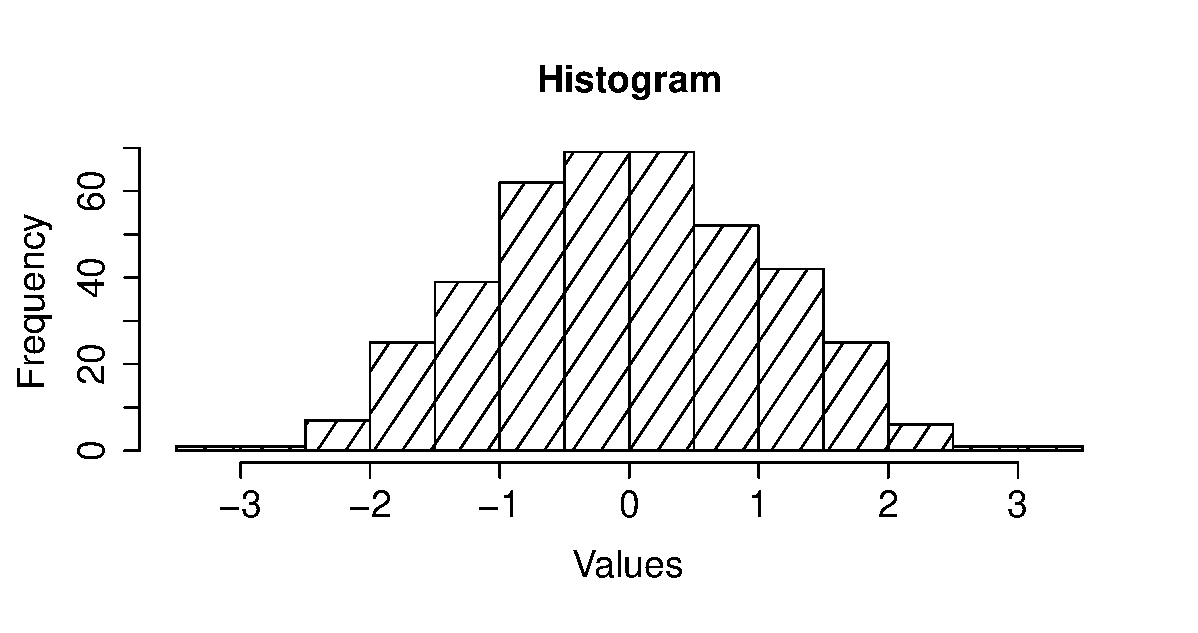
\includegraphics[width=0.8\textwidth, trim = 0.0cm 0.6cm 1.5cm 0.8cm, clip]{Hist}
\end{center}
{\bf Q4} Based on the above histogram, which of the following is likely to be true?\\[0.2cm]
\begin{tabular}{cccc}
{\bf(a)} $\bar x > Q_2$ & {\bf(b)} $\bar x < Q_2$ & {\bf(c)} $\bar x \approx \mu$  & {\bf(d)} $\bar x \approx Q_2$ \\[0.6cm]
\end{tabular}


\rule{\linewidth}{1pt}

\quad\\
Consider the following sample of ages of mechanical components:
\begin{center}
\begin{tabular}{|cccccc|}
\hline
&&&&&\\[-0.4cm]
5 & 1 & 6 & 5 & 5 & 3\\
\hline
\multicolumn{6}{c}{}
\end{tabular}
\end{center}

{\bf Q5} What is the value of the standard deviation for this sample?\\[0.2cm]
\begin{tabular}{cccc}
{\bf(a)} $s = 1.83$ years & {\bf(b)} $s^2 = 3.37$ years$^2$ & {\bf(c)} $s = 2.43$ years & {\bf(d)} $\sigma = 1.83$ years \\[0.6cm]
\end{tabular}

\quad

\rule{\linewidth}{1pt}

\newpage

\section*{Rough Work\\[23cm]}
\section*{\hspace{8cm}$\boxed{\text{Next page: Questions 6 - 10}}$}

\newpage


\section*{Questions 6 - 10}

\rule{\linewidth}{1pt}

\begin{center}
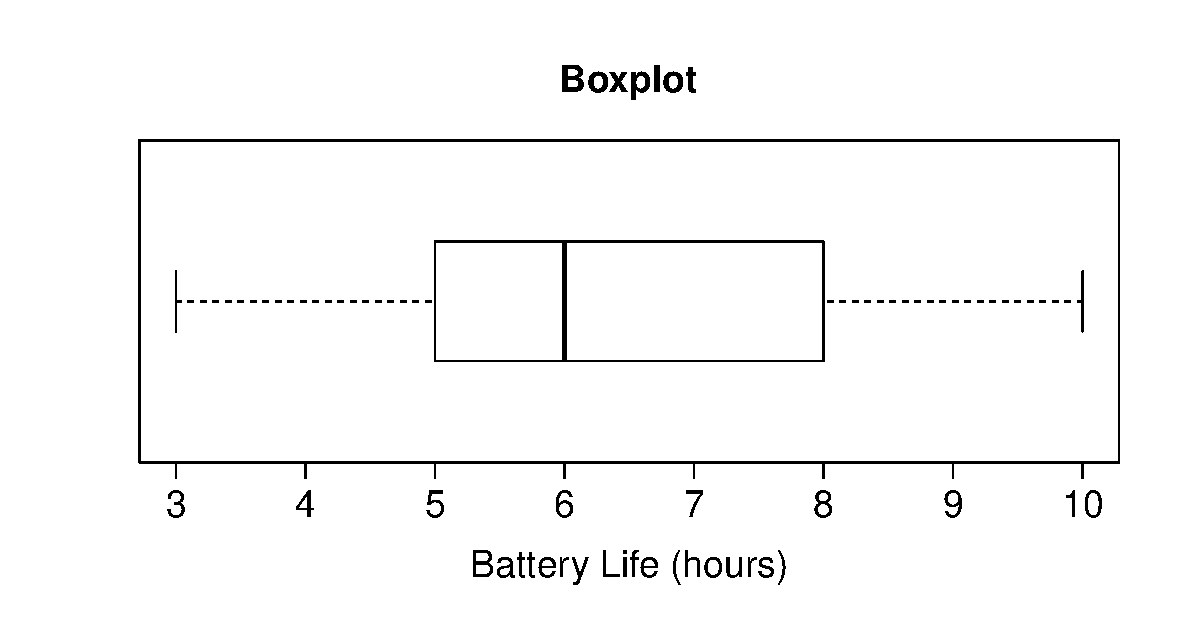
\includegraphics[width=0.8\textwidth, trim = 1.3cm 0.6cm 1cm 0.8cm, clip]{Boxplot}
\end{center}

{\bf Q6} Based on the above boxplot, what is the value of the $IQR$?\\[0.2cm]
\begin{tabular}{cccc}
{\bf(a)} $3$ hours & {\bf(b)} $7$ hours & {\bf(c)} $1$ hour & {\bf(d)} 2 hours \\[0.6cm]
\end{tabular}

\rule{\linewidth}{1pt}
\quad\\
Consider the following set of numbers:
\begin{center}
\begin{tabular}{|ccccccccc|}
\hline
&&&&&&&&\\[-0.4cm]
13 & 5 & 21 & 11 & 15 & 13 & 12 & 14 & 8 \\
\hline
\multicolumn{9}{c}{}
\end{tabular}
\end{center}

{\bf Q7} What is the value of the median?\\[0.2cm]
\begin{tabular}{cccc}
{\bf(a)} 12.5 & {\bf(b)} 5 & {\bf(c)} 13 & {\bf(d)} 15 \\[0.6cm]
\end{tabular}

{\bf Q8} How many outliers are there?\\[0.2cm]
\begin{tabular}{cccc}
{\bf(a)} 0 & {\bf(b)} 1 & {\bf(c)} 2 & {\bf(d)} 3 \\[0.6cm]
\end{tabular}

\rule{\linewidth}{1pt}
\quad\\
{\bf Q9} Let $\Pr(A) = 0.3$, $\Pr(B) = 0.6$ and $\Pr(A \cap B) = 0.25$. What is the value of $\Pr(A^c \cap B^c)$? \\[0.2cm]
\begin{tabular}{cccc}
{\bf(a)} 0.1 & {\bf(b)} 0.28 & {\bf(c)} 0.35 & {\bf(d)} 0.75 \\[0.6cm]
\end{tabular}


\rule{\linewidth}{1pt}
\quad\\
Consider a random number generator which assigns a value to $X$ according to the following probability distribution:
\begin{center}
\begin{tabular}{|c|cccc|}
\hline
&&&&\\[-0.4cm]
$x$        & 0 & 2 & 4 & 10 \\
\hline
&&&&\\[-0.4cm]
$\Pr(X=x)$ & 0.3 & 0.5 & 0.1 & ? \\
\hline
\multicolumn{5}{c}{}
\end{tabular}
\end{center}

{\bf Q10} What is the value of $E(X)$?\\[0.2cm]
\begin{tabular}{cccc}
{\bf(a)} 0.1 & {\bf(b)} 2.4 & {\bf(c)} 1.4 & {\bf(d)} 2.8 \\[0.6cm]
\end{tabular}

\rule{\linewidth}{1pt}

\newpage

\section*{Rough Work\\[23cm]}
\section*{\hspace{8cm}$\boxed{\text{Next page: Questions 11 - 15}}$}

\newpage

\section*{Questions 11 - 15}


\rule{\linewidth}{1pt}
\quad\\
{\bf Q11} You have 10 t-shirts. You're going on holidays and can only bring 4 of them. How many possible groups of 4 t-shirts are there if one of them is your ``lucky'' t-shirt and you \emph{must} bring it?\\[0.2cm]
\begin{tabular}{cccc}
{\bf(a)} 210 & {\bf(b)} 504 & {\bf(c)} 120 & {\bf(d)} 84 \\[0.6cm]
\end{tabular}



\rule{\linewidth}{1pt}
\quad\\
A laptop manufacturer uses two types of keyboard: Type-1 is used 80\% of the time and Type-2 is used 20\% of the time. It is known that 10\% of Type-1 keyboards are faulty and 30\% of Type-2 keyboards are faulty.\\[0.3cm]

{\bf Q12} What is the probability that a randomly selected keyboard will be faulty?\\[0.2cm]
\begin{tabular}{cccc}
{\bf(a)} 0.19 & {\bf(b)} 0.4 & {\bf(c)} 0.26 & {\bf(d)} 0.14 \\[0.6cm]
\end{tabular}

{\bf Q13}  A keyboard is tested and found to be \emph{working}; what is the probability that it is Type-1?\\[0.2cm]
%{\footnotesize(answer is given to two decimal places)}\\[0.2cm]
\begin{tabular}{cccc}
{\bf(a)} 0.9 & {\bf(b)} 0.57 & {\bf(c)} 0.84 & {\bf(d)} 0.16 \\[0.6cm]
\end{tabular}





\rule{\linewidth}{1pt}
\quad\\
There is a 5\% chance of pressing the wrong button on a keyboard and thus make a typographical error. Assuming these errors occur independently, the number of errors in typing $n$ letters is $X \sim$ Binomial$(n,p)$.\\[0.3cm]

{\bf Q14} You type 12 letters. What is the probability of making \emph{less than} 2 errors? \\[0.2cm]
%{\footnotesize(hint: cannot use tables)}\\[0.2cm]
\begin{tabular}{cccc}
{\bf(a)} 0.3413 & {\bf(b)} 0.8816 & {\bf(c)} 0.9804 & {\bf(d)} 0.0988 \\[0.6cm]
\end{tabular}

{\bf Q15} You type 100 letters. What is $\Pr(X > 10)$? \\[0.2cm]
%{\footnotesize(hint: use tables)}\\[0.2cm]
\begin{tabular}{cccc}
{\bf(a)} 0.0282 & {\bf(b)} 0.0167  & {\bf(c)} 0.0115 & {\bf(d)} 0.0072 \\[0.6cm]
\end{tabular}

\rule{\linewidth}{1pt}








\newpage

\section*{Rough Work\\[23cm]}
\section*{\hspace{2cm}$\boxed{\text{Don't forget to enter your answers on the last page!}}$}

\newpage


\section*{Useful Formulae: Page 1\\[0.3cm]}
{\bf Histogram:}\\[-0.8cm]
\begin{align*}
\bullet\quad \text{class width} = \frac{\max(x) - \min(x)}{\text{number of classes}}\\
\end{align*}
{\bf Numerical Summaries:}\\[-0.8cm]
\begin{align*}
\bullet\quad \bar x &= \frac{\sum\,x_i}{n}\\[0.6cm]
\bullet\quad s^2 &= \frac{\sum\,x_i^2 - n\,\bar x^2}{n-1}\\[0.6cm]
\bullet\quad \text{Position of } Q_k:& \quad \frac{n+1}{4}\times k \\[0.6cm]
\bullet\quad IQR &= Q_3 - Q_1 \\[0.6cm]
\bullet\quad LF &= Q_1 - 1.5 \times IQR \\[0.6cm]
\bullet\quad UF &= Q_3 + 1.5 \times IQR\\
\end{align*}
{\bf Probability:}\\[-0.8cm]
\begin{align*}
\bullet\quad \Pr(A^c) &= 1 - \Pr(A) \\[1cm]
\bullet\quad \Pr(A \cup B) &= \Pr(A) + \Pr(B) - \Pr(A \cap B)\\[0.6cm]
\bullet\quad \Pr(E_1 \cup E_2 \cup \cdots \cup E_k) &= \Pr(E_1) + \Pr(E_2) + \cdots + \Pr(E_k) \text{\quad{\footnotesize(if mutually exclusive)}}\\[1cm]
\bullet\quad \Pr(A \cap B) &= \Pr(A) \, \Pr(B \, | \, A) = \Pr(B) \, \Pr(A \, | \, B) \\[0.6cm]
\bullet\quad \Pr(E_1 \cap E_2 \cap \cdots \cap E_k) &= \Pr(E_1) \, \Pr(E_2) \, \cdots \, \Pr(E_k) \text{\quad{\footnotesize(if independent)}}\\[1cm]
\bullet\quad \Pr(A\,|\,B) &= \frac{\Pr(A \cap B)}{\Pr(B)} = \frac{\Pr(A) \,\Pr(B\,|\,A)}{\Pr(B)}\\[1cm]
\bullet\quad \text{If $E_1,\ldots, E_k$} & \,\, \text{are mutually exclusive \& exhaustive}\\[0.1cm]
\Rightarrow \Pr(B) &= \Pr(B \cap E_1) + \Pr(B \cap E_2) + \cdots + \Pr(B \cap E_k) \\[0.2cm]
&= \Pr(E_1) \, \Pr(B\,|\,E_1) + \Pr(E_2) \, \Pr(B\,|\,E_2) + \cdots + \Pr(E_k) \, \Pr(B\,|\,E_k)\\
\end{align*}

\newpage

\section*{Useful Formulae: Page 2\\[0.3cm]}
{\bf Counting Techniques:}\\[-0.8cm]
\begin{align*}
\bullet\quad n\,! &= n\times(n-1)\times(n-2)\times\cdots\times3\times2\times 1\\[0.6cm]
\bullet\quad \binom{n}{k} &= \frac{n\,!}{k\,! (n-k)\,!}\\
\end{align*}
{\bf Random Variables:}\\[-0.8cm]
\begin{align*}
\bullet\quad E(X) &= \sum x_i \,\, p(x_i)\\[0.6cm]
\bullet\quad E(X^2) &= \sum x_i^2 \,\, p(x_i)\\[0.6cm]
\bullet\quad Var(X) &= E(X^2) - [E(X)]^2\\[0.6cm]
\bullet\quad Sd(X) &= \sqrt{Var(X)}\\
\end{align*}
{\bf Binomial Distribution:}\\[-0.8cm]
\begin{align*}
\bullet\quad X &\sim \text{Binomial}(n,p)\\[0.6cm]
\bullet\quad \Pr(X=x) &= \binom{n}{x}\,p^x\,(1-p)^{n-x}\\[0.6cm]
\bullet\quad x &\in \{0,1,2,\ldots,n\}\\[0.6cm]
\bullet\quad E(X) &= n\,p \\[0.6cm]
\bullet\quad Var(X) &= n\,p\,(1-p)\\
\end{align*}

\newpage


\begin{adjustwidth}{-1cm}{0cm}
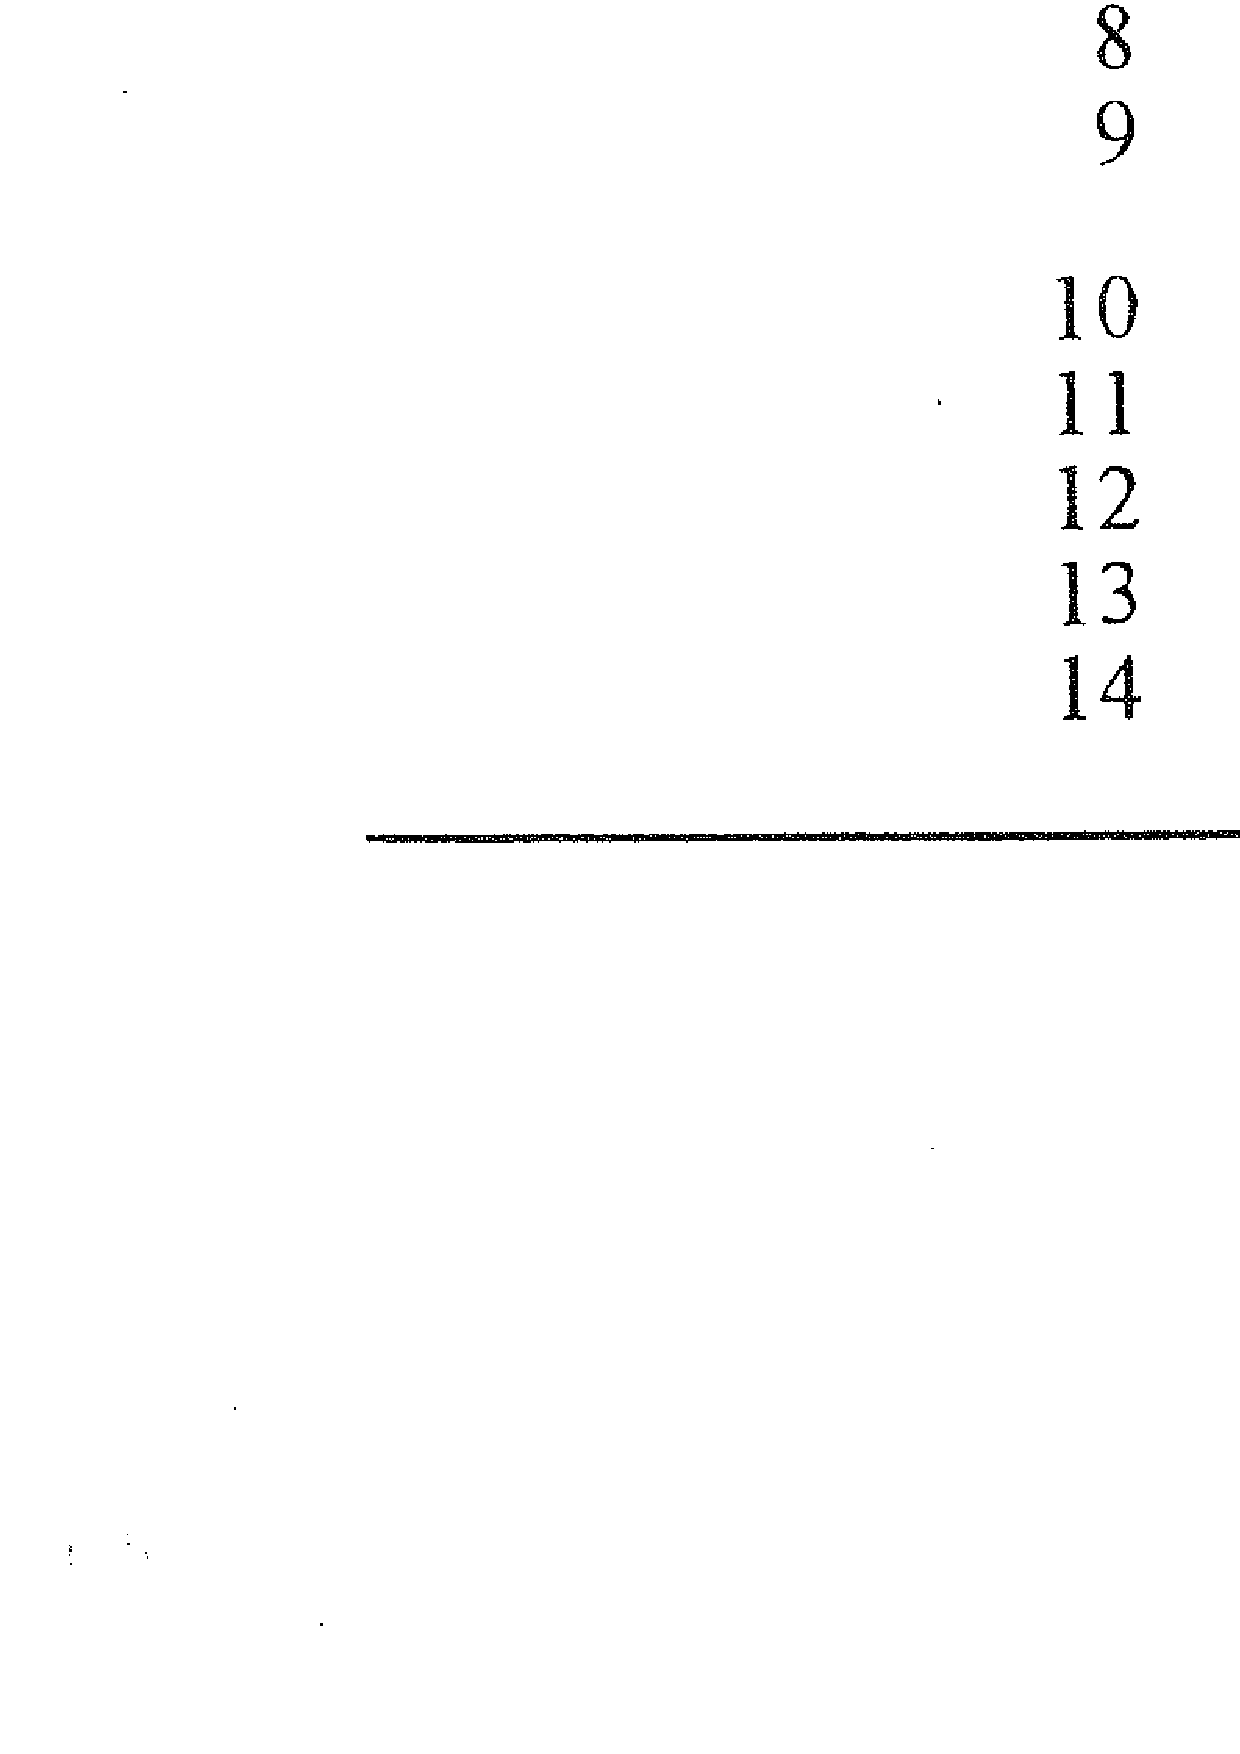
\includegraphics[width=1.1\textwidth, trim = 2cm 4cm 2cm 3cm, clip]{Md1}
\end{adjustwidth}

\newpage

\begin{adjustwidth}{-1cm}{0cm}
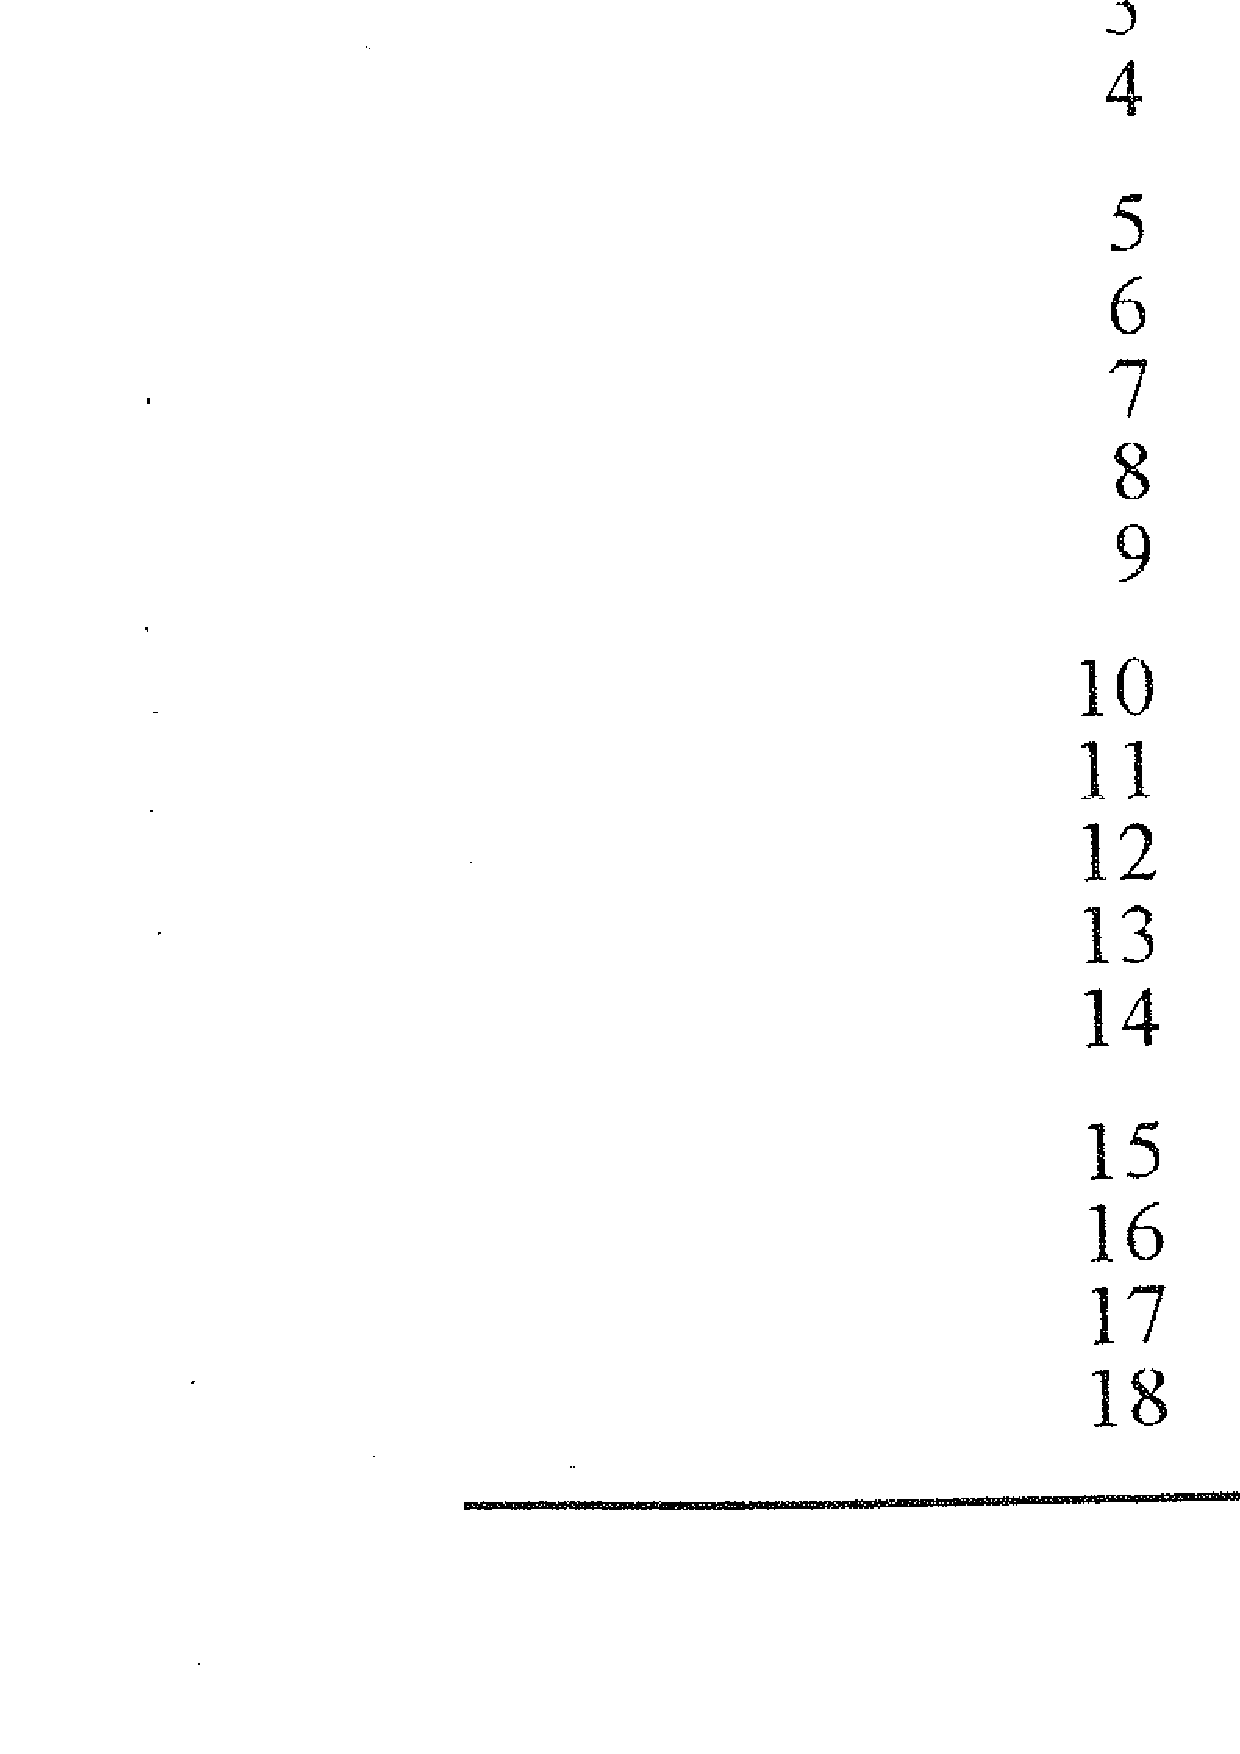
\includegraphics[width=1.1\textwidth, trim = 2cm 4cm 2cm 3cm, clip]{Md2}
\end{adjustwidth}

\newpage

\section*{Answer Sheet\\[0.3cm]}

\subsection*{Name:\quad\underline{\hspace{11.45cm}}\\[0.3cm]}
\subsection*{ID Number:\quad\underline{\hspace{10cm}}\\[0.5cm]}

Enter your answers with an ``X' in the table below.\\[0.3cm]
Do not enter the ``X'' until you have made your \emph{final decision} to avoid scribbling out.\\[0.3cm]
\begin{large}
\begin{center}
\begin{tabular}{|c|c|c|c|c|}
\hline
&&&&\\[-0.4cm]
 & A & B & C & D \\
\hline
&&&&\\[-0.4cm]
Q1 &&&& \\
\hline
&&&&\\[-0.4cm]
Q2 &&&& \\
\hline
&&&&\\[-0.4cm]
Q3 &&&& \\
\hline
&&&&\\[-0.4cm]
Q4 &&&& \\
\hline
&&&&\\[-0.4cm]
Q5 &&&& \\
\hline
\multicolumn{5}{c}{}\\[-0.3cm]
\hline
&&&&\\[-0.4cm]
Q6 &&&& \\
\hline
&&&&\\[-0.4cm]
Q7 &&&& \\
\hline
&&&&\\[-0.4cm]
Q8 &&&& \\
\hline
&&&&\\[-0.4cm]
Q9 &&&& \\
\hline
&&&&\\[-0.4cm]
Q10 &&&& \\
\hline
\multicolumn{5}{c}{}\\[-0.3cm]
\hline
&&&&\\[-0.4cm]
Q11 &&&& \\
\hline
&&&&\\[-0.4cm]
Q12 &&&& \\
\hline
&&&&\\[-0.4cm]
Q13 &&&& \\
\hline
&&&&\\[-0.4cm]
Q14 &&&& \\
\hline
&&&&\\[-0.4cm]
Q15 &&&& \\
\hline
\end{tabular}
\end{center}
\end{large}


\end{document} 